\documentclass[tikz,border=6pt]{standalone}
\usepackage{tikz}
\usetikzlibrary{arrows.meta, positioning, fit}

\definecolor{cGreen}{HTML}{84c960}
\definecolor{cGold}{HTML}{e7bc58}
\definecolor{cTeal}{HTML}{416473}

\begin{document}
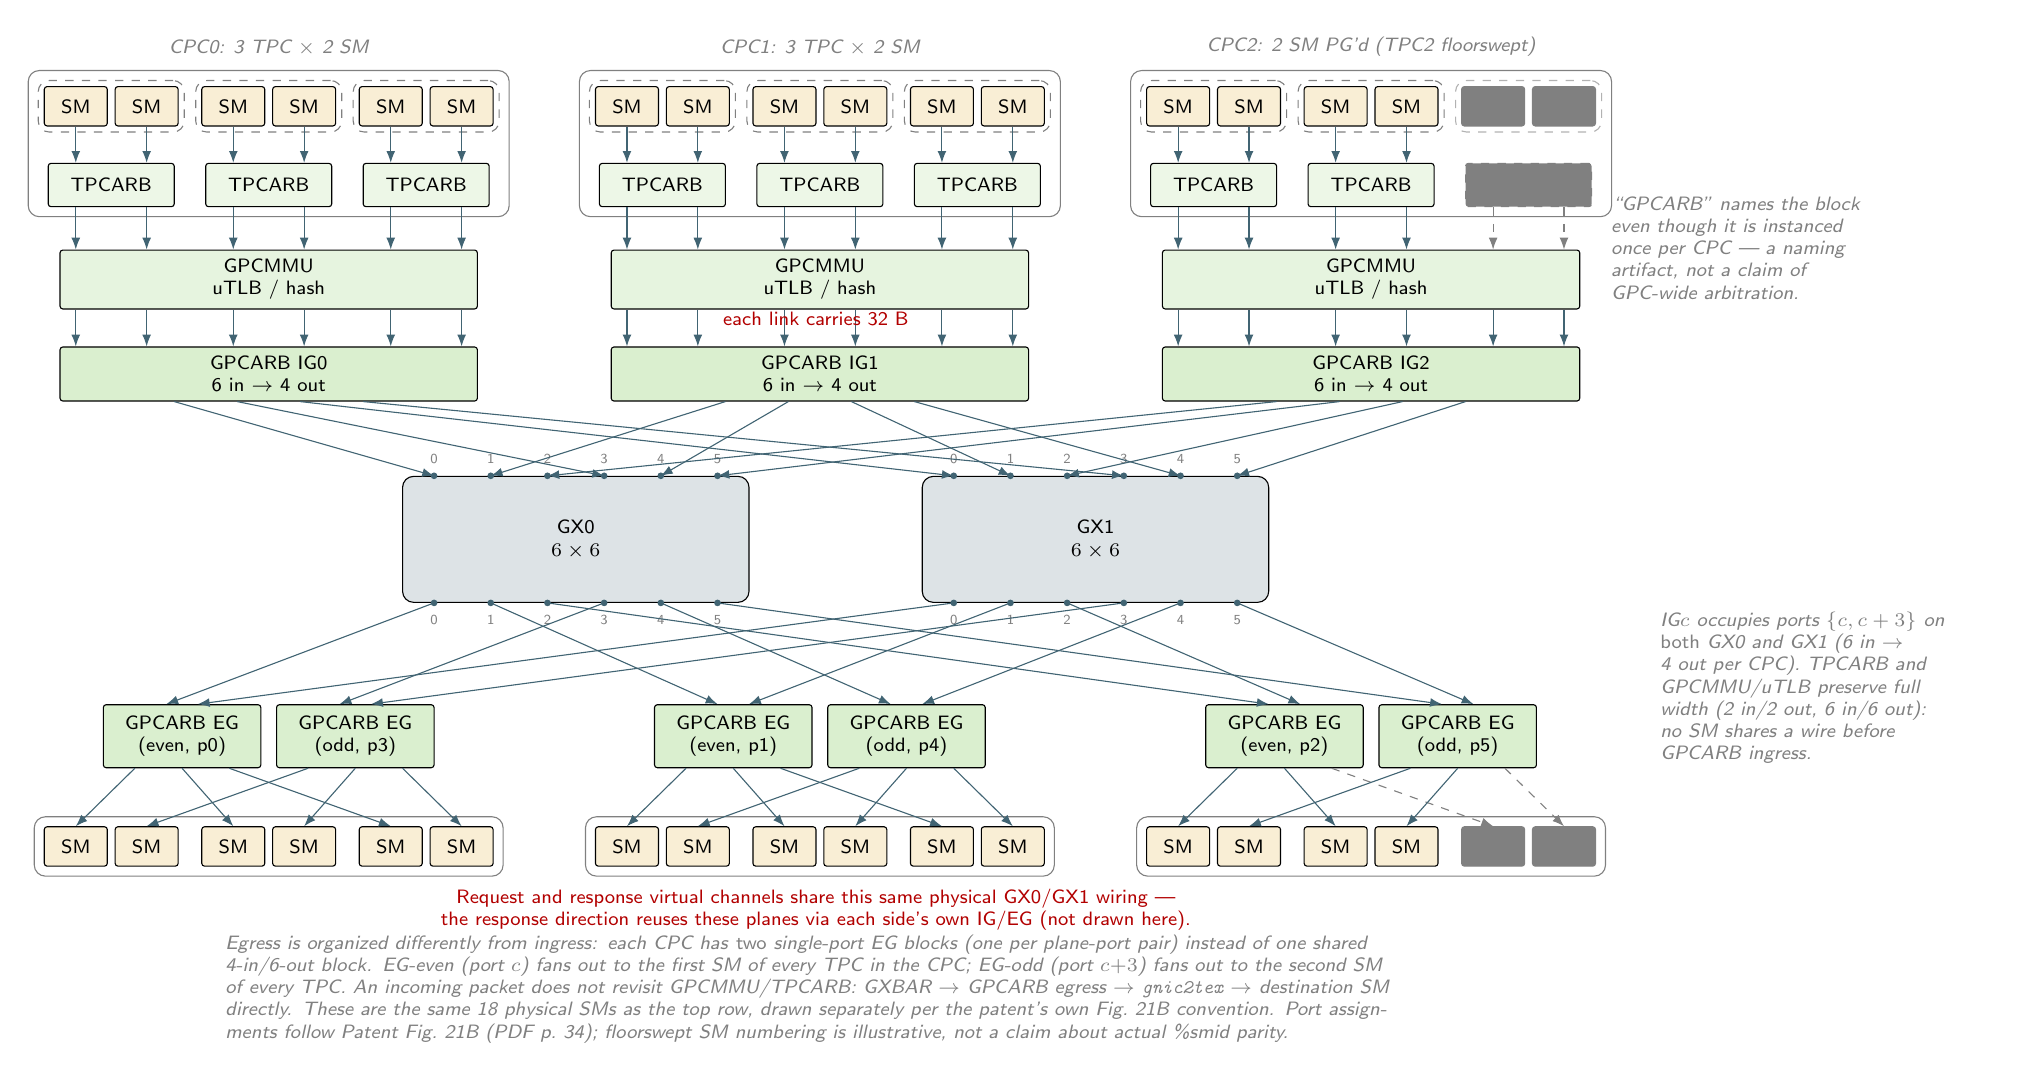
\begin{tikzpicture}[
  font=\sffamily\scriptsize,
  sm/.style={draw, rounded corners=1pt, minimum width=8mm, minimum height=5mm,
             align=center, fill=cGold!25, font=\sffamily\scriptsize},
  smoff/.style={draw, gray, rounded corners=1pt, minimum width=8mm, minimum height=5mm,
             align=center, fill=gray!12, font=\sffamily\scriptsize, gray},
  tpc/.style={draw, dashed, gray, rounded corners, inner sep=0.7mm},
  tpcoff/.style={draw, dashed, gray!60, rounded corners, inner sep=0.7mm},
  cpc/.style={draw, gray, rounded corners, inner sep=1.2mm},
  arb/.style={draw, rounded corners=1pt, minimum width=16mm, minimum height=5.5mm,
              align=center, fill=cGreen!15, font=\sffamily\scriptsize},
  arboff/.style={draw, gray, dashed, rounded corners=1pt, minimum width=16mm,
                 minimum height=5.5mm, align=center, fill=gray!10,
                 font=\sffamily\scriptsize, gray},
  utlb/.style={draw, rounded corners=1pt, minimum width=53mm, minimum height=6mm,
               align=center, fill=cGreen!20, font=\sffamily\scriptsize},
  ig/.style={draw, rounded corners=1pt, minimum width=53mm, minimum height=6mm,
             align=center, fill=cGreen!30, font=\sffamily\scriptsize},
  eg/.style={draw, rounded corners=1pt, minimum width=20mm, minimum height=8mm,
             align=center, fill=cGreen!30, font=\sffamily\scriptsize},
  gx/.style={draw, rounded corners, minimum width=44mm, minimum height=16mm,
             align=center, fill=cTeal!18, font=\sffamily\scriptsize},
  port/.style={circle, fill=cTeal, inner sep=0.3mm},
  portlbl/.style={font=\sffamily\tiny, gray},
  lane/.style={-{Latex[length=1.5mm]}, thin, color=cTeal},
  laneoff/.style={-{Latex[length=1.5mm]}, thin, color=gray, dashed},
  lbl/.style={font=\sffamily\scriptsize\itshape, align=center, gray},
]

%% the 6 wire columns of one CPC, as x-offsets from the CPC's own center
%% (matches the 3 TPCARB centers +/-4.5mm, i.e. exactly under each SM)
\def\sixOff{-24.5,-15.5,-4.5,4.5,15.5,24.5}
%% the 6 GX port x-offsets from a GX plane's own center (ports 0..5, left to right)
\def\portOffA{-18} \def\portOffB{-10.8} \def\portOffC{-3.6}
\def\portOffD{3.6}  \def\portOffE{10.8}  \def\portOffF{18}

%% ================= SRC side: CPC0/CPC1, y = 60 down to 26 =================
\foreach \cpc/\base/\lbltext in {0/0/{CPC0: 3 TPC $\times$ 2 SM},
                                  1/70/{CPC1: 3 TPC $\times$ 2 SM}} {
  \foreach \t/\tx in {0/0, 1/20, 2/40} {
    \pgfmathsetmacro{\gx}{\base+\tx}
    \node[sm] (c\cpc_t\t_s0) at (\gx mm, 60mm) {SM};
    \node[sm] (c\cpc_t\t_s1) at (\gx mm + 9mm, 60mm) {SM};
    \node[tpc, fit=(c\cpc_t\t_s0)(c\cpc_t\t_s1)] (c\cpc_tpc\t) {};
    \node[arb] (c\cpc_arb\t) at (\gx mm + 4.5mm, 50mm) {TPCARB};
    \draw[lane] (c\cpc_t\t_s0.south) -- (c\cpc_arb\t.north -| c\cpc_t\t_s0.south);
    \draw[lane] (c\cpc_t\t_s1.south) -- (c\cpc_arb\t.north -| c\cpc_t\t_s1.south);
  }
  \node[cpc, fit=(c\cpc_tpc0)(c\cpc_tpc2)(c\cpc_arb0)(c\cpc_arb2)] (cpc\cpc srcbox) {};
  \node[lbl, above=0.5mm of cpc\cpc srcbox] {\lbltext};
  \node[utlb] (c\cpc_utlb) at (\base mm + 24.5mm, 38mm) {GPCMMU\\uTLB / hash};
  \foreach \t/\tx in {0/0, 1/20, 2/40} {
    \draw[lane] (c\cpc_arb\t.south -| c\cpc_t\t_s0.south) -- (c\cpc_utlb.north -| c\cpc_t\t_s0.south);
    \draw[lane] (c\cpc_arb\t.south -| c\cpc_t\t_s1.south) -- (c\cpc_utlb.north -| c\cpc_t\t_s1.south);
  }
  \node[ig] (c\cpc_ig) at (\base mm + 24.5mm, 26mm) {GPCARB IG\cpc\\6 in $\to$ 4 out};
  \foreach \o in \sixOff {
    \draw[lane] ([xshift=\o mm]c\cpc_utlb.south) -- ([xshift=\o mm]c\cpc_ig.north);
  }
}

%% ---- CPC2 (base 140), TPC2 floorswept ----
\foreach \t/\tx in {0/140, 1/160} {
  \node[sm] (c2_t\t_s0) at (\tx mm, 60mm) {SM};
  \node[sm] (c2_t\t_s1) at (\tx mm + 9mm, 60mm) {SM};
  \node[tpc, fit=(c2_t\t_s0)(c2_t\t_s1)] (c2_tpc\t) {};
  \node[arb] (c2_arb\t) at (\tx mm + 4.5mm, 50mm) {TPCARB};
  \draw[lane] (c2_t\t_s0.south) -- (c2_arb\t.north -| c2_t\t_s0.south);
  \draw[lane] (c2_t\t_s1.south) -- (c2_arb\t.north -| c2_t\t_s1.south);
}
\node[smoff] (c2_t2_s0) at (180mm, 60mm) {SM};
\node[smoff] (c2_t2_s1) at (189mm, 60mm) {SM};
\node[tpcoff, fit=(c2_t2_s0)(c2_t2_s1)] (c2_tpc2) {};
\node[arboff] (c2_arb2) at (184.5mm, 50mm) {TPCARB};
\node[cpc, fit=(c2_tpc0)(c2_tpc2)(c2_arb0)(c2_arb2)] (cpc2box) {};
\node[lbl, above=0.5mm of cpc2box] {CPC2: 2 SM PG'd (TPC2 floorswept)};
\node[utlb] (c2_utlb) at (164.5mm, 38mm) {GPCMMU\\uTLB / hash};
\draw[lane] (c2_arb0.south -| c2_t0_s0.south) -- (c2_utlb.north -| c2_t0_s0.south);
\draw[lane] (c2_arb0.south -| c2_t0_s1.south) -- (c2_utlb.north -| c2_t0_s1.south);
\draw[lane] (c2_arb1.south -| c2_t1_s0.south) -- (c2_utlb.north -| c2_t1_s0.south);
\draw[lane] (c2_arb1.south -| c2_t1_s1.south) -- (c2_utlb.north -| c2_t1_s1.south);
\draw[laneoff] (c2_arb2.south -| c2_t2_s0.south) -- (c2_utlb.north -| c2_t2_s0.south);
\draw[laneoff] (c2_arb2.south -| c2_t2_s1.south) -- (c2_utlb.north -| c2_t2_s1.south);
\node[ig] (c2_ig) at (164.5mm, 26mm) {GPCARB IG2\\6 in $\to$ 4 out};
\foreach \o in \sixOff {
  \draw[lane] ([xshift=\o mm]c2_utlb.south) -- ([xshift=\o mm]c2_ig.north);
}

\node[lbl, align=left, text width=48mm] at (219mm, 42mm)
  {``GPCARB'' names the block\\even though it is instanced\\once per CPC --- a naming\\artifact, not a claim of\\GPC-wide arbitration.};

%% ================= GXBAR: two wide 6x6 planes, 6 explicit ports each side =================
\node[gx] (gx0) at (63.5mm, 5mm) {GX0\\$6\times6$};
\node[gx] (gx1) at (129.5mm, 5mm) {GX1\\$6\times6$};
\foreach \g in {gx0, gx1} {
  \foreach \i/\o in {0/\portOffA, 1/\portOffB, 2/\portOffC, 3/\portOffD, 4/\portOffE, 5/\portOffF} {
    \node[port] at ([xshift=\o mm]\g.north) {};
    \node[portlbl, above=0.3mm] at ([xshift=\o mm]\g.north) {\i};
    \node[port] at ([xshift=\o mm]\g.south) {};
    \node[portlbl, below=0.3mm] at ([xshift=\o mm]\g.south) {\i};
  }
}

%% IG_c's 4 outputs -> GX0 ports {c,c+3} and GX1 ports {c,c+3}
% CPC0: ports 0,3
\draw[lane] ([xshift=-12mm]c0_ig.south) -- ([xshift=\portOffA mm]gx0.north);
\draw[lane] ([xshift=-4mm]c0_ig.south)  -- ([xshift=\portOffD mm]gx0.north);
\draw[lane] ([xshift=4mm]c0_ig.south)   -- ([xshift=\portOffA mm]gx1.north);
\draw[lane] ([xshift=12mm]c0_ig.south)  -- ([xshift=\portOffD mm]gx1.north);
% CPC1: ports 1,4
\draw[lane] ([xshift=-12mm]c1_ig.south) -- ([xshift=\portOffB mm]gx0.north);
\draw[lane] ([xshift=-4mm]c1_ig.south)  -- ([xshift=\portOffE mm]gx0.north);
\draw[lane] ([xshift=4mm]c1_ig.south)   -- ([xshift=\portOffB mm]gx1.north);
\draw[lane] ([xshift=12mm]c1_ig.south)  -- ([xshift=\portOffE mm]gx1.north);
% CPC2: ports 2,5
\draw[lane] ([xshift=-12mm]c2_ig.south) -- ([xshift=\portOffC mm]gx0.north);
\draw[lane] ([xshift=-4mm]c2_ig.south)  -- ([xshift=\portOffF mm]gx0.north);
\draw[lane] ([xshift=4mm]c2_ig.south)   -- ([xshift=\portOffC mm]gx1.north);
\draw[lane] ([xshift=12mm]c2_ig.south)  -- ([xshift=\portOffF mm]gx1.north);

\node[lbl, anchor=north west, align=left, text width=44mm] at (200mm, -3mm)
  {IG$c$ occupies ports $\{c,c+3\}$ on\\\emph{both} GX0 and GX1 (6 in $\to$\\4 out per CPC). TPCARB and\\GPCMMU/uTLB preserve full\\width (2 in/2 out, 6 in/6 out):\\no SM shares a wire before\\GPCARB ingress.};

\node[font=\sffamily\scriptsize, color=red!70!black] at (94mm, 33mm)
  {each link carries 32 B};
\node[font=\sffamily\scriptsize, color=red!70!black, align=center, text width=150mm] at (94mm, -42mm)
  {Request and response virtual channels share this same physical GX0/GX1
   wiring --- the response direction reuses these planes via each side's
   own IG/EG (not drawn here).};

%% ================= DEST side: GX -> 2 GPCARB EG per CPC (even/odd port) -> 3 SM each =================
%% Per the patent (Fig. 21B), egress is NOT one 4-in/6-out block per CPC.
%% Each CPC has two single-port EG blocks: EG-even at port c, EG-odd at port c+3.
%% Each EG takes one line from GX0 and one from GX1 at its own port index,
%% and fans out to the same TPC-relative SM slot across all 3 TPCs.
\node[eg] (c0_ege) at (13.5mm, -20mm) {GPCARB EG\\(even, p0)};
\node[eg] (c0_ego) at (35.5mm, -20mm) {GPCARB EG\\(odd, p3)};
\node[eg] (c1_ege) at (83.5mm, -20mm) {GPCARB EG\\(even, p1)};
\node[eg] (c1_ego) at (105.5mm, -20mm) {GPCARB EG\\(odd, p4)};
\node[eg] (c2_ege) at (153.5mm, -20mm) {GPCARB EG\\(even, p2)};
\node[eg] (c2_ego) at (175.5mm, -20mm) {GPCARB EG\\(odd, p5)};

\draw[lane] ([xshift=\portOffA mm]gx0.south) -- ([xshift=-2mm]c0_ege.north);
\draw[lane] ([xshift=\portOffA mm]gx1.south) -- ([xshift=2mm]c0_ege.north);
\draw[lane] ([xshift=\portOffD mm]gx0.south) -- ([xshift=-2mm]c0_ego.north);
\draw[lane] ([xshift=\portOffD mm]gx1.south) -- ([xshift=2mm]c0_ego.north);
\draw[lane] ([xshift=\portOffB mm]gx0.south) -- ([xshift=-2mm]c1_ege.north);
\draw[lane] ([xshift=\portOffB mm]gx1.south) -- ([xshift=2mm]c1_ege.north);
\draw[lane] ([xshift=\portOffE mm]gx0.south) -- ([xshift=-2mm]c1_ego.north);
\draw[lane] ([xshift=\portOffE mm]gx1.south) -- ([xshift=2mm]c1_ego.north);
\draw[lane] ([xshift=\portOffC mm]gx0.south) -- ([xshift=-2mm]c2_ege.north);
\draw[lane] ([xshift=\portOffC mm]gx1.south) -- ([xshift=2mm]c2_ege.north);
\draw[lane] ([xshift=\portOffF mm]gx0.south) -- ([xshift=-2mm]c2_ego.north);
\draw[lane] ([xshift=\portOffF mm]gx1.south) -- ([xshift=2mm]c2_ego.north);

%% destination SMs: EG-even feeds the first SM of each TPC, EG-odd the second
\foreach \cpc/\base in {0/0, 1/70} {
  \foreach \t/\tx in {0/0, 1/20, 2/40} {
    \pgfmathsetmacro{\gx}{\base+\tx}
    \node[sm] (d\cpc_t\t_s0) at (\gx mm, -34mm) {SM};
    \node[sm] (d\cpc_t\t_s1) at (\gx mm + 9mm, -34mm) {SM};
  }
  \node[cpc, fit=(d\cpc_t0_s0)(d\cpc_t2_s1)] (dcpc\cpc dstbox) {};
}
\draw[lane] ([xshift=-6mm]c0_ege.south) -- (d0_t0_s0.north);
\draw[lane] ([xshift=0mm]c0_ege.south) -- (d0_t1_s0.north);
\draw[lane] ([xshift=6mm]c0_ege.south) -- (d0_t2_s0.north);
\draw[lane] ([xshift=-6mm]c0_ego.south) -- (d0_t0_s1.north);
\draw[lane] ([xshift=0mm]c0_ego.south) -- (d0_t1_s1.north);
\draw[lane] ([xshift=6mm]c0_ego.south) -- (d0_t2_s1.north);
\draw[lane] ([xshift=-6mm]c1_ege.south) -- (d1_t0_s0.north);
\draw[lane] ([xshift=0mm]c1_ege.south) -- (d1_t1_s0.north);
\draw[lane] ([xshift=6mm]c1_ege.south) -- (d1_t2_s0.north);
\draw[lane] ([xshift=-6mm]c1_ego.south) -- (d1_t0_s1.north);
\draw[lane] ([xshift=0mm]c1_ego.south) -- (d1_t1_s1.north);
\draw[lane] ([xshift=6mm]c1_ego.south) -- (d1_t2_s1.north);

\foreach \t/\tx in {0/140, 1/160} {
  \node[sm] (d2_t\t_s0) at (\tx mm, -34mm) {SM};
  \node[sm] (d2_t\t_s1) at (\tx mm + 9mm, -34mm) {SM};
}
\node[smoff] (d2_t2_s0) at (180mm, -34mm) {SM};
\node[smoff] (d2_t2_s1) at (189mm, -34mm) {SM};
\node[cpc, fit=(d2_t0_s0)(d2_t2_s1)] (dcpc2box) {};
\draw[lane] ([xshift=-6mm]c2_ege.south) -- (d2_t0_s0.north);
\draw[lane] ([xshift=0mm]c2_ege.south) -- (d2_t1_s0.north);
\draw[laneoff] ([xshift=6mm]c2_ege.south) -- (d2_t2_s0.north);
\draw[lane] ([xshift=-6mm]c2_ego.south) -- (d2_t0_s1.north);
\draw[lane] ([xshift=0mm]c2_ego.south) -- (d2_t1_s1.north);
\draw[laneoff] ([xshift=6mm]c2_ego.south) -- (d2_t2_s1.north);

\node[lbl, anchor=north, align=left, text width=150mm] at (94mm, -44mm)
  {Egress is organized differently from ingress: each CPC has \emph{two}
   single-port EG blocks (one per plane-port pair) instead of one shared
   4-in/6-out block. EG-even (port $c$) fans out to the first SM of every
   TPC in the CPC; EG-odd (port $c{+}3$) fans out to the second SM of every
   TPC. An incoming packet does not revisit GPCMMU/TPCARB: GXBAR
   $\rightarrow$ GPCARB egress $\rightarrow$ \texttt{gnic2tex} $\rightarrow$
   destination SM directly. These are the same 18 physical SMs as the top
   row, drawn separately per the patent's own Fig.~21B convention. Port
   assignments follow Patent Fig.~21B (PDF p.~34); floorswept SM numbering
   is illustrative, not a claim about actual \%smid parity.};

\end{tikzpicture}
\end{document}
